%_____________________________________________________________________________________________ 
% LATEX Template: Department of Comp/IT BTech Project Reports
% Sample Chapter
% Sun Mar 27 10:25:35 IST 2011
%
% Note: Itemization, enumeration and other things not shown. A sample figure is included.
%_____________________________________________________________________________________________ 

\chapter{System design criteria}
\section{Requirements}
The software is very lightweight and runs on a machine with bare minimum configuration. Following are the minimum software and hardware requirements for the program.
\subsection{Hardware requirements (Same as for Python platform)}
\begin{itemize}
\item Memory/RAM : 512MB.
\item Hard Disk Space : 1GB.
\item Processor : Intel Pentium 4 or later.
\end{itemize}

\subsection{Software requirements}
\begin{itemize}
\item Operating system: GNU/Linux or Windows
\item Python (v2.7)
\item Libraries: Wxpython, Wxwidgets
\item Python modules: pickle, ezodf, pdfkit
\end{itemize}

\section{Constraints}
Constraints are the rules that must be satisfied by the timetable. Hard constraints are the ones which can not be violated. Soft constraints can be violated but generates warnings.
\subsection{Hard constraints}
\begin{enumerate}
\item No clashes in \textit{teacher} / \textit{venue} / \textit{class} / \textit{batch} timetable.
\item Allocated hours of a subject in timetable should not exceed the no of hours allocated to it by the institute.
\end{enumerate}

\subsection{Soft constraints}
\begin{enumerate}
\item \textit{Teacher's} workload should not exceed maximum(max) \textit{teacher} workload.
\item \textit{Venue} capacity should be greater than or equal to \textit{class} capacity.
\item Compulsory lunch break for each \textit{class} / \textit{batch}.
\item Allocated hours for a \textit{subject} in timetable should not be less than no of hours allocated to it by the institute. 
\end{enumerate}

\newpage
\section{Approach of design}
\textit{Teacher, Venue and Classes} are the three classes that are central to the working of application. Every individual teacher, venue or class is an instance of one of these classes. User needs to input data i.e. list of teachers, venues, classes and subjects. This data can also be imported from external files. Given below is the format of data that should be followed.


\begin{table}[h!]
\centering
\begin{tabular}{|l|c|c|c|}

\hline
Teacher Name & Abbreviation & WeeklyMaxLoad & DailyMaxLoad\\
\hline
Abhijit A M & AM & 25 & 5\\
\hline
Satish Kumbhar & SSK & 28 & 5\\
\hline
Jibi Abraham & JA & 22 & 5\\
\hline
\end{tabular}
\caption{Teacher Table}
\label{tab:template}
\end{table}

\begin{table}[h!]
\centering
\begin{tabular}{|l|c|c|}

\hline
 Class Name & Abbreviation & Size\\
\hline
SYComp & SYC & 75\\
\hline
TYComp & TYC & 75\\
\hline 
\end{tabular}
\caption{Class Table}
\label{tab:template}
\end{table}

\begin{table}[h!]
\centering
\begin{tabular}{|l|c|c|}

\hline
Subject Name & Abbreviation & No of hours\\
\hline
DataStructure & DSA & 4\\
\hline
MathI & M1 & 4\\
\hline 
\end{tabular}
\caption{Subject Table}
\label{tab:template}
\end{table}


\begin{table}[h!]
\centering
\begin{tabular}{|l|c|c|}

\hline
 Venue Name & Abbreviation & Capacity\\
\hline
Academic Complex 201 & AC201 & 120\\
 \hline
Academic Complex 302 & AC302 & 120\\
\hline 
\end{tabular}
\caption{Class Table}
\label{tab:template}
\end{table}


% \begin{figure}[ht!]
% 	\centering
% 	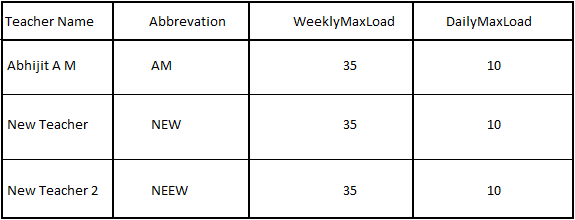
\includegraphics[width=140mm]{teacher.png}
% 	\caption{Teacher Data}
% \end{figure}

% \begin{figure}[ht!]
% 	\centering
% 	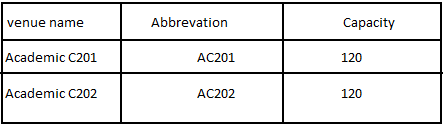
\includegraphics[width=110mm]{venue.png}
% 	\caption{Venue Data}
% \end{figure}

% \begin{figure}[ht!]
% 	\centering
% 	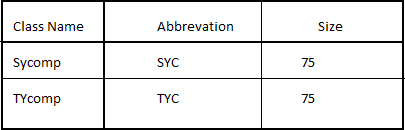
\includegraphics[width=120mm]{class.png}
% 	\caption{Class Data}
% \end{figure}

% \newpage
% \begin{figure}[ht!]
% 	\centering
% 	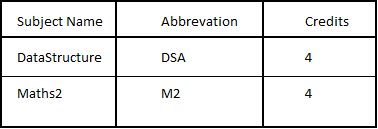
\includegraphics[width=100mm]{subject.png}
% 	\caption{Subject Data}
% \end{figure}

When user adds an entry in any of the timetable it is verified against all existing entries for violation of constraints. The change is allowed only after verification, failing which all changes are discarded. During this, constraints like teacher's work load, number of hours allocated to the subject are also checked. Venue capacity is verified for every venue-class pair. After an entry is successfully added teacher work load and subject hour count is incremented. When a hard constraint is violated all changes are discarded and an error is shown immediately. When a soft constraint is violated the warning is added to global warning section. User can view or manage global warnings any time from the menubar.



\subsection{List of Features}
\noindent
\begin{itemize}
\item Support for batches.
\item Individual teacher work load.
\item Venue-class capacity checking.
\item Venue utilization statistics.
\item Check all constraints function.
\item Pop-up box for input with dropdown suggestions.
\item Mapping and filter data in pop up box.
\item Direct typing in cell for input.
\item Mandatory lunch breaks.
\item Cut-paste / copy-paste.
\item Support for standard keyboard functions - enter, delete, backspace.
\item Import data from files.
\item Export \textit{pdf}, \textit{html} and \textit{ods}.
\item Open project with cmd argument. 
\item Save / open project.
\item Merge / unmerge selected cells.
\item Delete entry.
\item Warning list for soft constraint violation.
\item Number of hours for subject, teacher workload and venue capacity / class size changeable at runtime.

\end{itemize}
%_____________________________________________________________________________________________ 
 
 
